\documentclass[aspectratio=169]{beamer}
\usepackage{multicol}
\usepackage{qrcode}
\usepackage{datetime}
\usepackage{hyperref}
\usepackage{xcolor}
\usepackage{tikz}

\usetheme{Antibes}
\setbeamertemplate{footline}[frame number]{}

\newcommand{\makemycolor}[2]{%
    \pgfmathsetmacro{\hue}{(#1/100)^1.715*0.79}%
    \definecolor{myhsbcolor}{hsb}{\hue,1,1}%
    \textcolor{myhsbcolor}{#2}%
}

\hypersetup{
    colorlinks=true,
    linkcolor=blue,
    filecolor=magenta,      
    urlcolor=blue,
    pdftitle={La Rete Bitcoin},
    pdfpagemode=FullScreen,
    }

\urlstyle{same}

\title{La Rete Bitcoin} 
\author{Valerio Vaccaro}
\newdate{date}{26}{02}{2024}
\date{\displaydate{date}}
\logo{}

\begin{document}

\begin{frame}[plain,noframenumbering]
    \titlepage
    \begin{center}
        
\includegraphics[height=1cm]{logo.png}
    \end{center}
\end{frame}

\begin{frame}[noframenumbering]
    \tableofcontents
\end{frame}

\begin{frame}{Chi sono?}
    \begin{multicols}{2}
        \begin{itemize}
            \item \href{https://t.me/valeriovaccaro}{Valerio Vaccaro}
            \item C64
            \item Laureato al Politecnico ...
            \item ... poi ci ho anche lavorato per 9 anni
            \item Hoya
            \item ...
        \end{itemize}
        
        \begin{itemize}
            \item ...
            \item Eternity wall
            \item EU Blockhackathon 2018
            \item Blockstream
            \item Satoshi Spritz
            \item Officine Bitcoin
        \end{itemize}
    \end{multicols} 
\end{frame}

\begin{frame}{Meme}
    \begin{center}
        
\includegraphics[height=5cm]{meme_1.jpg}
    \end{center}
    * entro la fine del corso capirete tutti i meme.
\end{frame}

\section{Introduzione a Bitcoin}

\begin{frame}{Da dove tutto ha avuto inizio}
    31 Ottobre 2008
    \begin{center}
        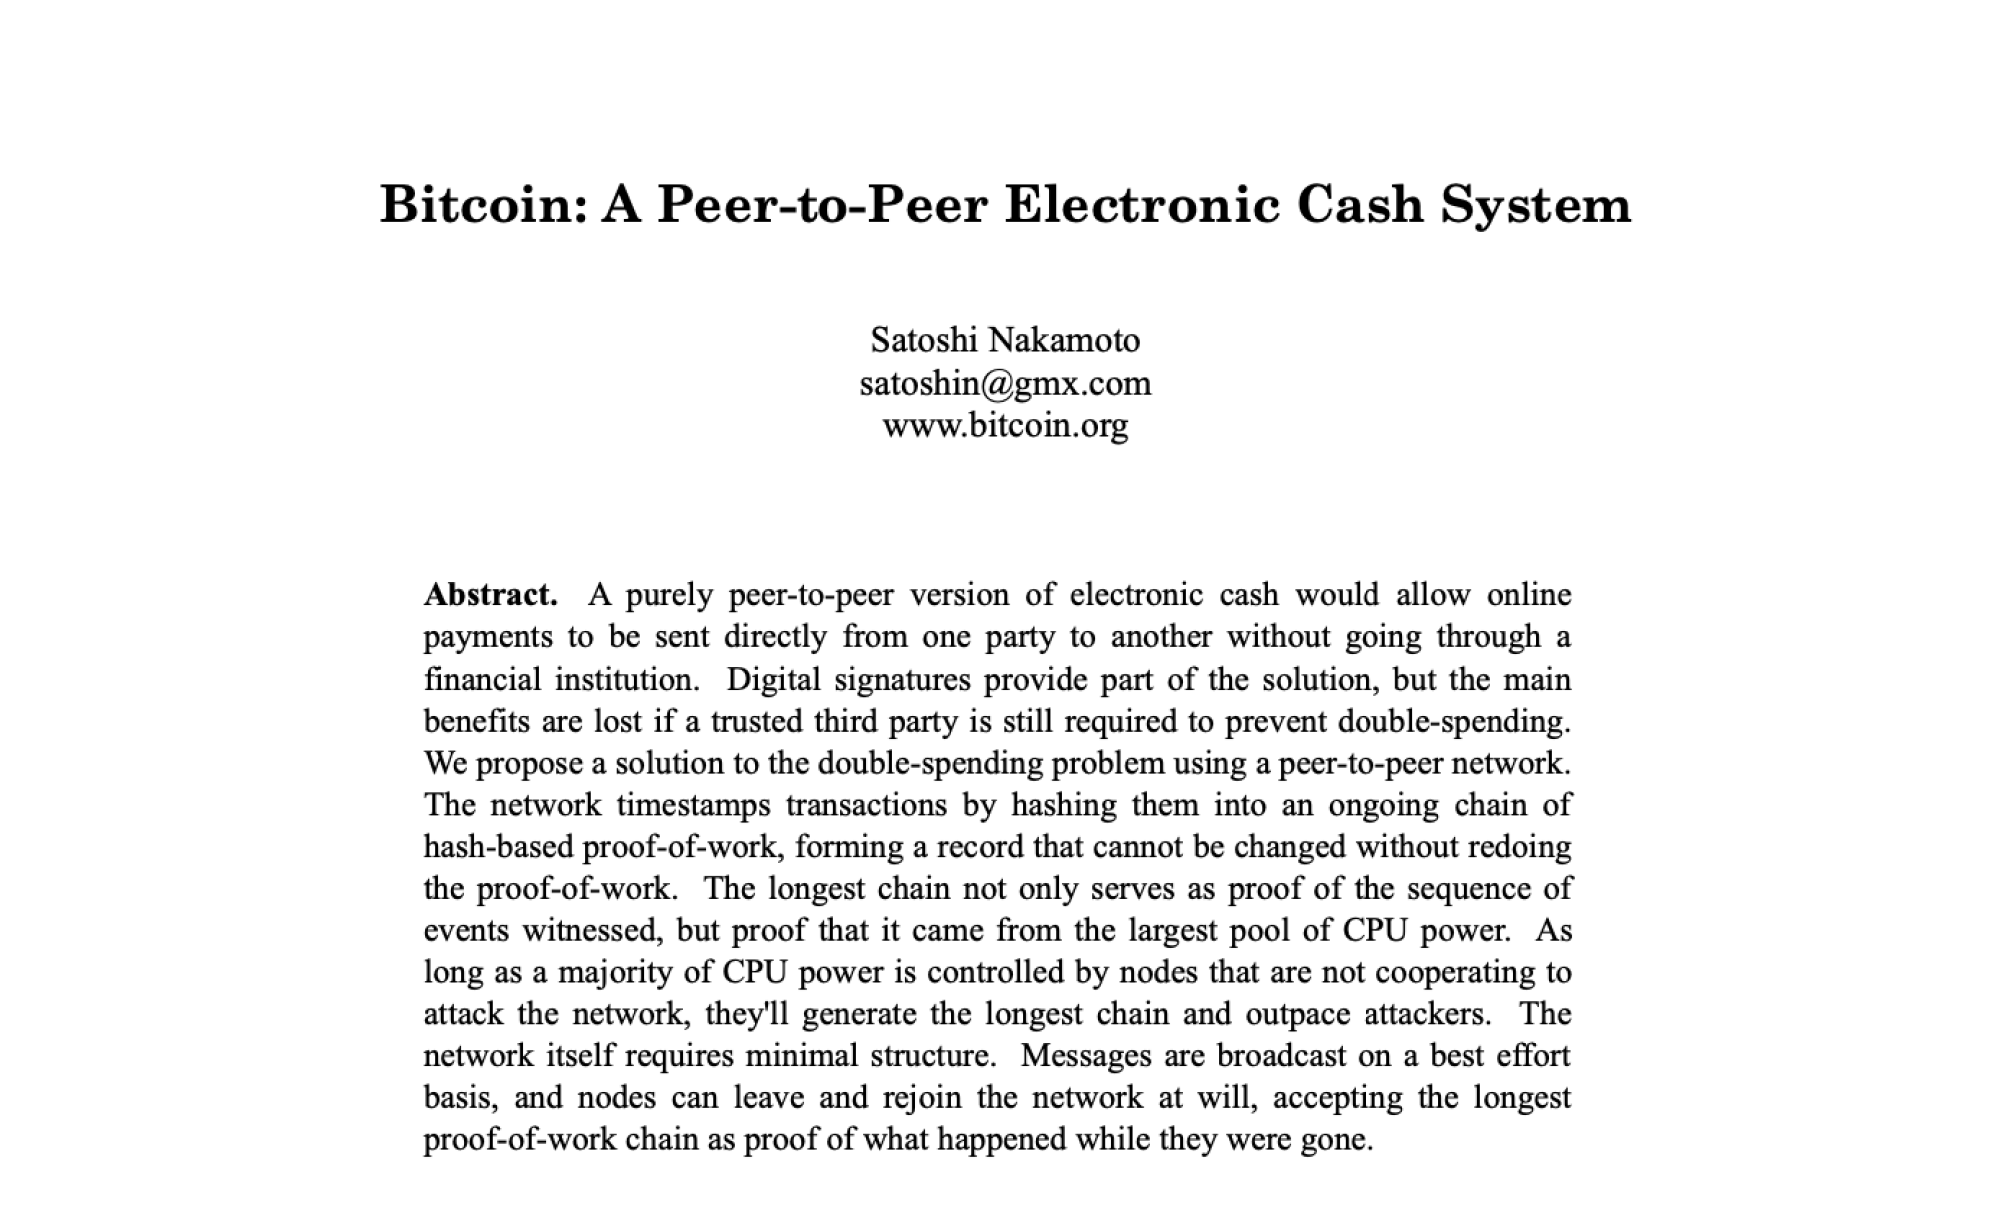
\includegraphics[height=5cm]{whitepaper.png}
    \end{center}
    La partenza della blockchain di Bitcoin avviene il 3 Gennaio 2009.
\end{frame}

\begin{frame}{Caratteristiche di Bitcoin}
    "Bitcoin è una raccolta di concetti e tecnologie che formano le basi per un
    ecosistema di denaro digitale. Le unità di valuta chiamate bitcoin vengono utilizzate
    per immagazzinare e trasferire valore tra i partecipanti del network Bitcoin."

    -- Mastering Bitcoin

    (tutta questa presentazione sarà fortemente basata su questo libro)
\end{frame}

\begin{frame}{Caratteristiche di Bitcoin}
    \begin{itemize}
        \item Denaro programmabile
        \item Totalmente distribuito
        \item Supply limitata (e no premine)
        \item Pseudo-anonimo
        \item Open-source
        \item Founder anonimo
        \item First-mover
        \item Grande e forte community
        \item ...
    \end{itemize}
    Unico nel panorama. 
\end{frame}

\section{Architettura Peer-to-Peer e consenso decentralizzato}

\begin{frame}{Reti Peer-to-Peer}
    Bitcoin è una rete peer-to-peer che non ha server centrali o architetture gerarchiche di controllo.
    
    Tutti i nodi sono uguali e contribuiscono a formare l'infrastruttura di rete di Bitcoin.

    Ritengo valide solo le informazioni che provengono dal \makemycolor{0}{mio} nodo.

    \begin{block}{Consenso}
        Le regole di validazione delle informazioni provenienti da altri nodi sono il \makemycolor{0}{consenso}, il mio nodo controlla il rispetto di tali regole.
    \end{block}

\end{frame}

\begin{frame}{Rete Bitcoin}
    I nodi sono pensati per funzionare in ogni contesto e specialmente nelle situazioni più critiche.

    \begin{itemize}
        \item Minimo consumo di risorse (o quantomento compatibile con hardware "casalingo")
        \item Minimo consumo di banda (funzionamento anche con reti mobili)
        \item Ridondanza della rete
        \item Robustezza del software
        \item ...
    \end{itemize}

    Grazie e queste sue caratteristiche è possibile mettersi un nodo in casa ed usarlo direttamente.
\end{frame}

\begin{frame}{Rete Bitcoin}
    Le funzionalità base dei nodi sono:

    \begin{itemize}
        \item Network Routing Node
        \item Full blockchain
        \item Wallet 
        \item Miner
    \end{itemize}
\end{frame}

\begin{frame}{Reti Bitcoin}
    Ma ci sono anche software aggiuntivi che permetto tanto altro.

    \begin{itemize}
        \item Indicizzatori
        \item Timestamping
        \item Colored coin 
        \item Second layer
        \item Sidechain
    \end{itemize}

    \begin{alertblock}{Opentimestamps}
        Ad esempio Opentimestamps è una architettura di server pubblici per l'attribuzione di una data certa ed immodificabile a qualsiasi documento digitale (anche a questa presentazione).
    \end{alertblock}

\end{frame}

\begin{frame}{Reti Bitcoin}
    \begin{center}
        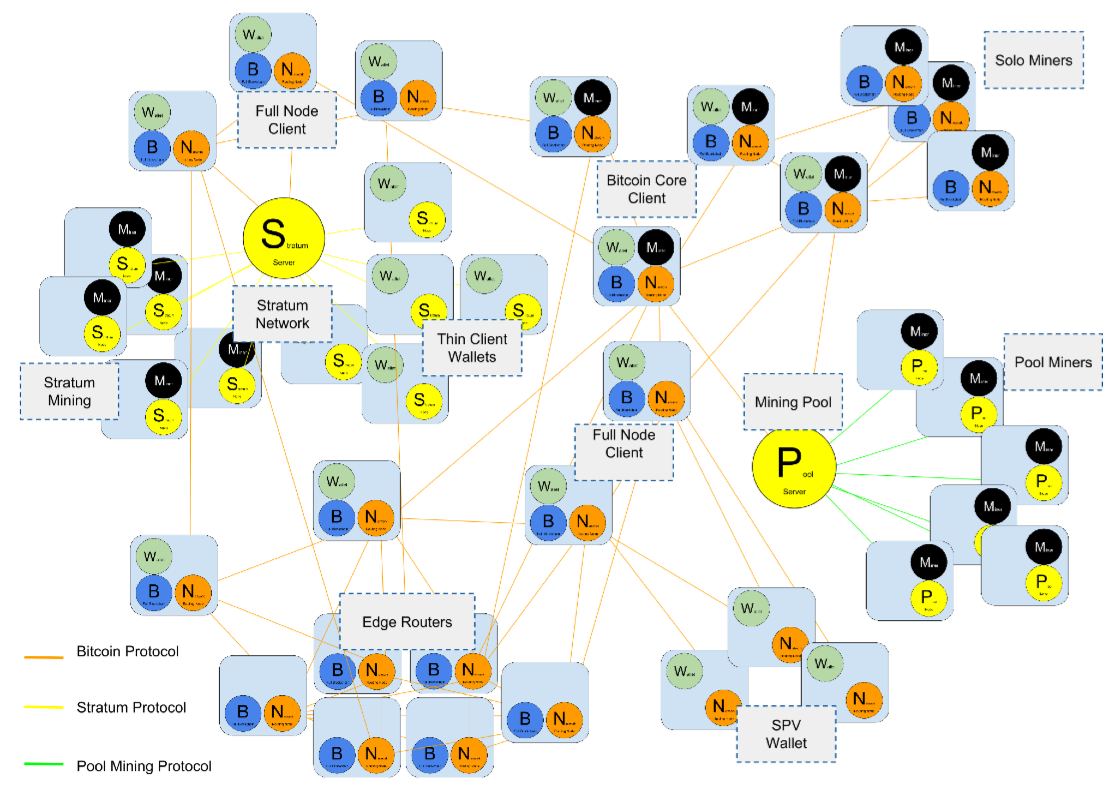
\includegraphics[height=5cm]{nodi.png}
    \end{center}
\end{frame}

\begin{frame}{Reti Bitcoin}
    \begin{center}
        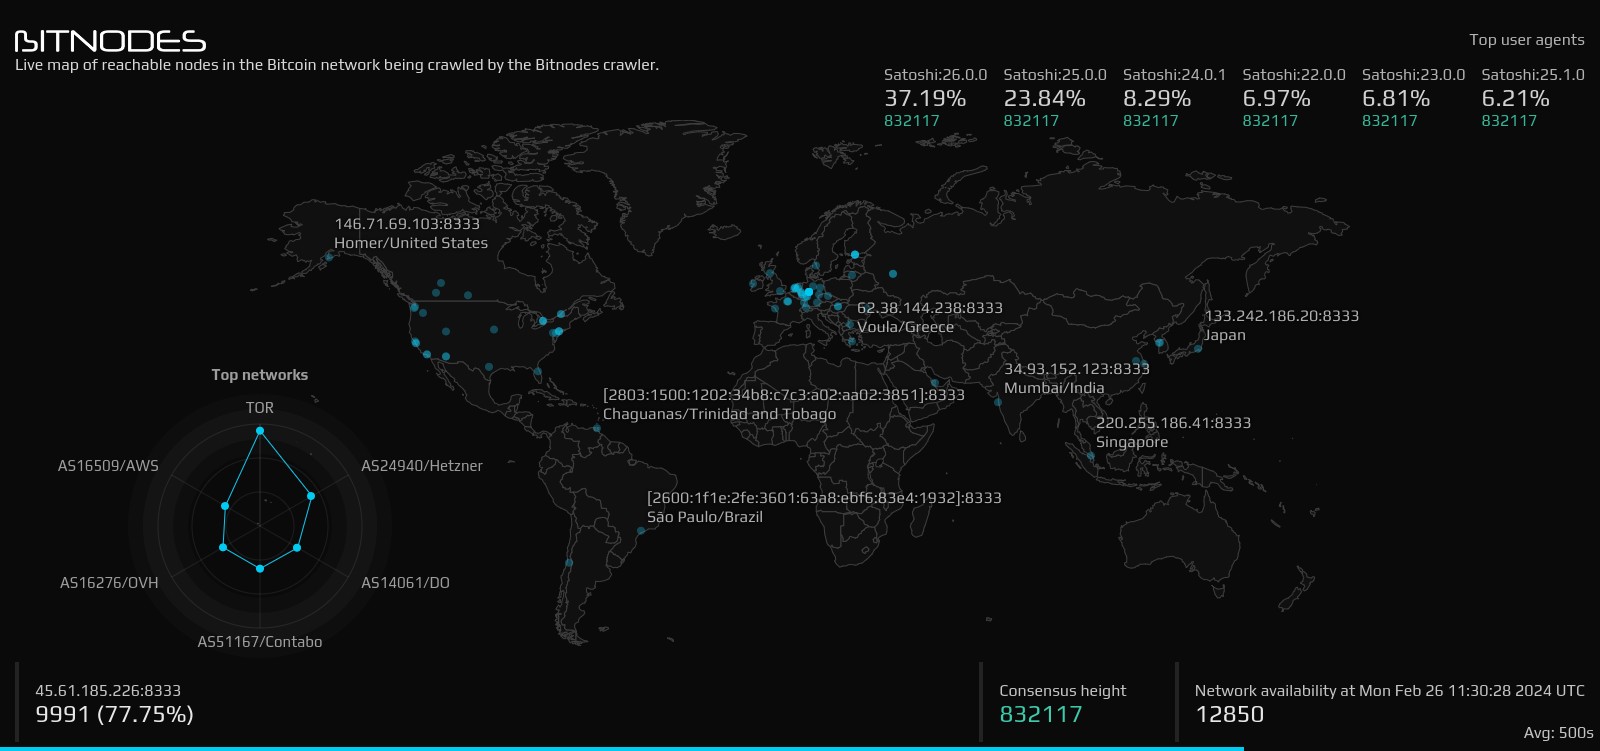
\includegraphics[height=5cm]{nodi_2.png}
    \end{center}
\end{frame}

\begin{frame}{Protocollo P2P}
    Il protocollo P2P alla base di Bitcoin ha subito varie trasformazioni al fine di incrementare le performance (soprattutto temporali) della rete.

    Il protocollo di discovery si basa su alcuni nodi noti (contattabili tramite specifici DNS) e da un protocollo di propagazione dell'identità ad altri nodi.

    Il nostro nodo quindi si connetterà ad un subset di tutti i nodi della rete.
\end{frame}

\begin{frame}{Protocollo P2P}
    Prosegue poi scaricando gli header dei blocchi e poi il contenuto dei blocchi stessi.

    \begin{center}
        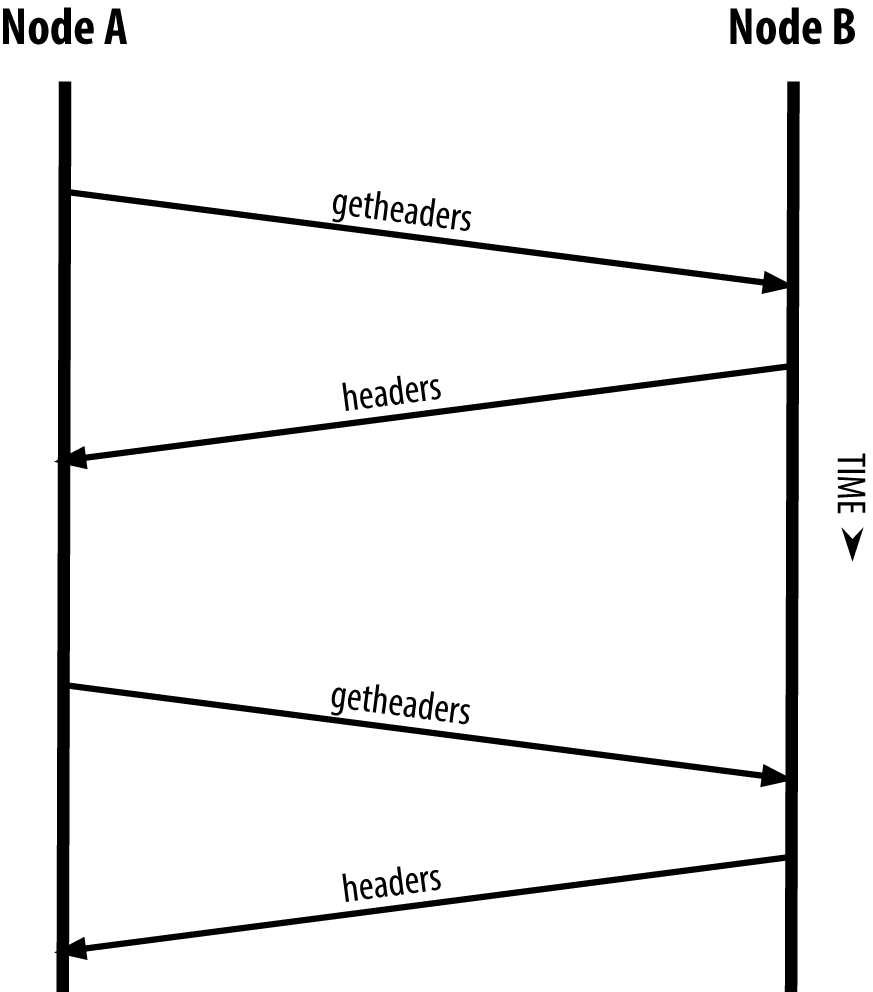
\includegraphics[height=5cm]{headers.png}
    \end{center}

    Fino ad aver scaricato e \makemycolor{0}{validato} tutti i blocchi.
\end{frame}

\begin{frame}{Protocollo P2P}
    \begin{center}
        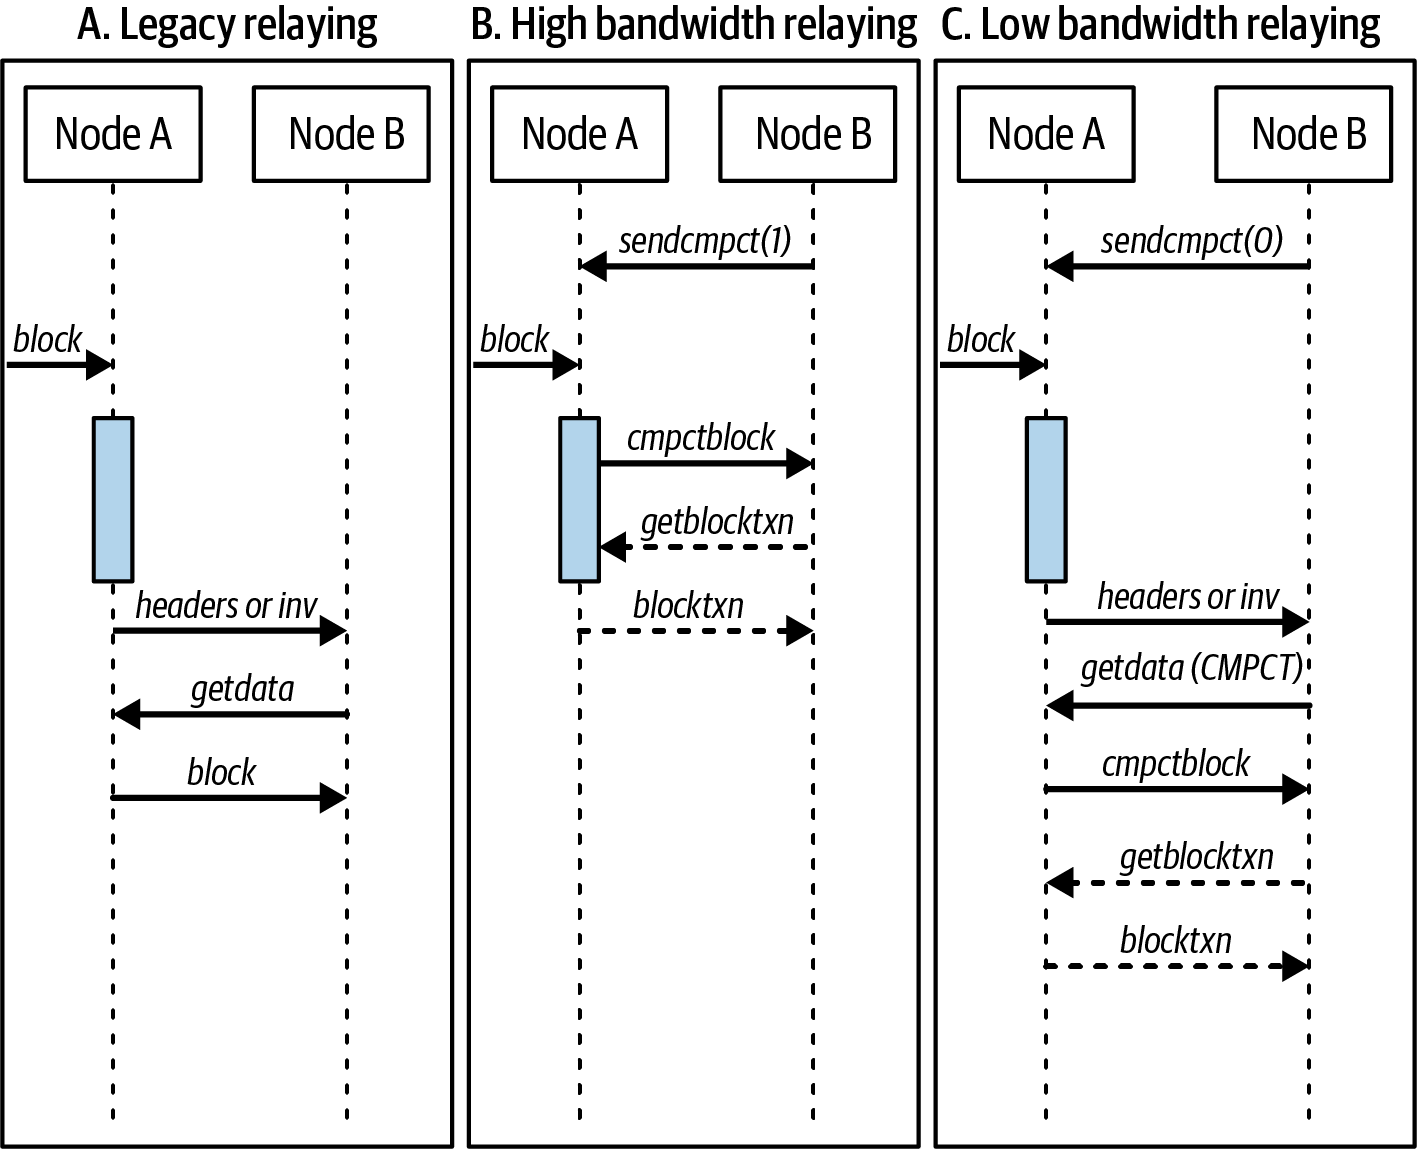
\includegraphics[height=5cm]{fullnode.png}
    \end{center}
\end{frame}

\section{Bitcoin Full Node: verifica indipendente delle transazioni e utilizzo dedicato}

\begin{frame}{Full node}
    I full node sono i nodi che contengono la copia completa di tutte le transazioni effettuate su Bitcoin.

    Questo consente di:
    \begin{itemize}
        \item identificare le transazioni ricevute
        \item verificare l'esistenza dei fondi ricevuti
    \end{itemize}

    Ma non tutti i wallet sono capaci di avere a bordo un fullnode.
\end{frame}

\section{Nodi di Simplified Payment Verification (SPV)}

\begin{frame}{SPV}
    Simple Payment verification è un protocollo che consente di validare le transazioni senza avere copia delle blockchain completa.

    I nodi SPV scaricano solo la lista degli header e poi chiedono ad altri full node una prova matematica della presenza di una certa transazione in un certo blocco.
\end{frame}

\section{Cosa sono e come funzionano i Bloom Filters}

\begin{frame}{Bloom Filters}
    I Bloom Filter sono una modalità per chiedere informazioni su un transazioni senza rivelare troppe informazioni su di essa.

    Consentono di richiedere informazioni ad un nodo SPV senza dire esplicitamente cosa si stà cercardo, i nodi hanno indici basati su questi filtri e possono rispondere più velocemente (ma ovviamente riveleranno più informazioni di quelle necessarie).
\end{frame}

\begin{frame}{Bloom Filters}
    \begin{center}
        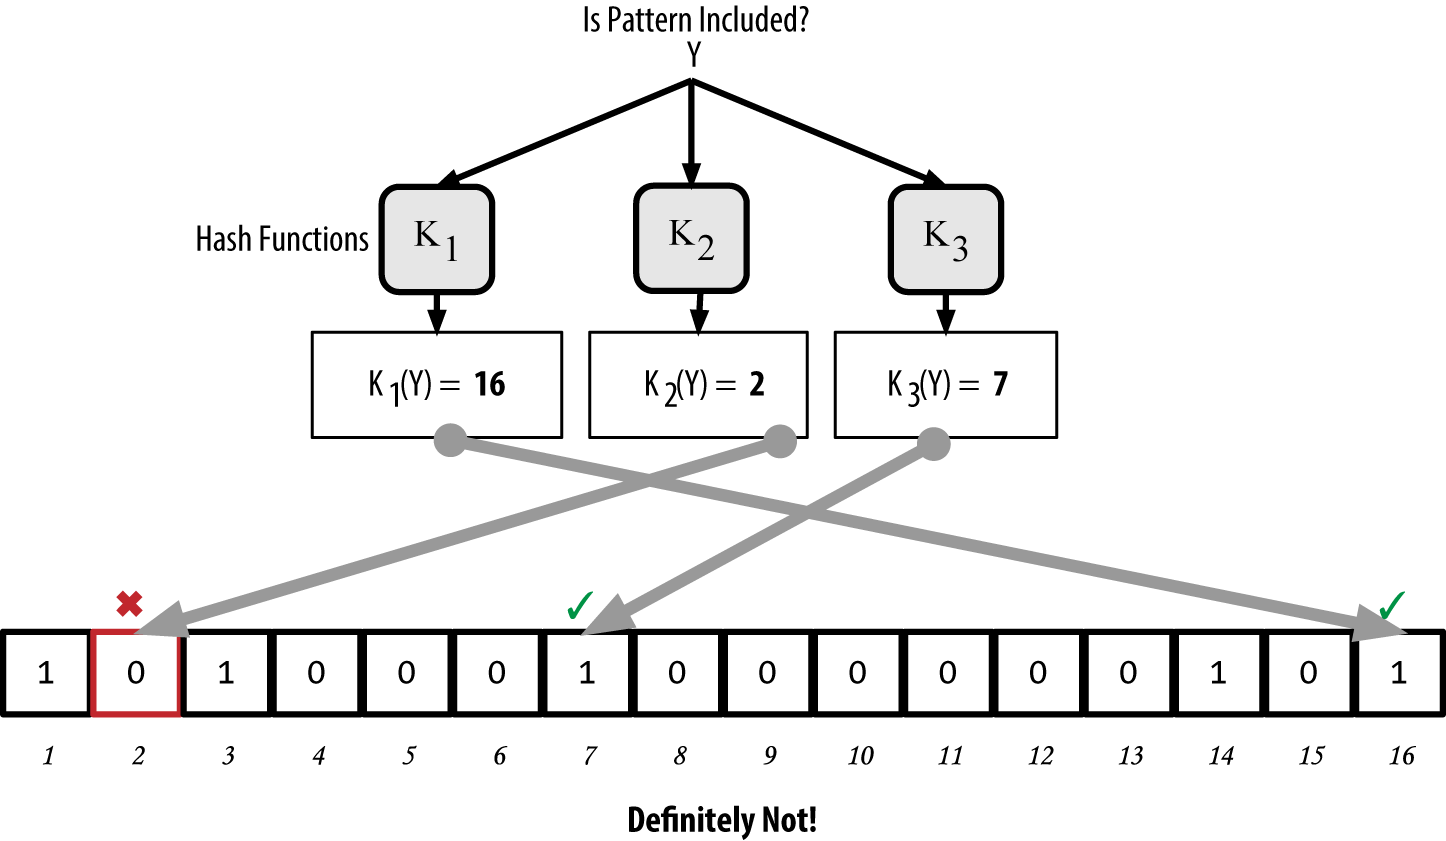
\includegraphics[height=5cm]{filter.png}
    \end{center}
\end{frame}

\section{Tor Transpor, Autenticazione e Crittografia Peer-to-Peer (BIP-150 e BIP-151)}

\begin{frame}{Tor}
    "Tor (acronimo di The Onion Router) è un software libero, rilasciato su licenza BSD 3-Clause, che permette una navigazione anonima sul Web ed è basato sulla terza generazione del protocollo di rete di onion routing: tramite il suo utilizzo è molto più difficile tracciare o intercettare l'attività che l'utente compie su Internet, sia da parte di società commerciali che da parte di soggetti potenzialmente ostili."

    \begin{alertblock}{DDOS}
        Tor è sotto un lunghissimo attacco DDOS! Potrebbe essere estremamente lento.
    \end{alertblock}
\end{frame}

\begin{frame}{BIP-150, BIP-151, ...}
    BIP-150 e BIP-151 sono proposte per autenticare e crittare la comunicazione tra diversi nodi Bitcoin. 

    BIP-324 ha proposto ed implementato (a partire da Bitcoin Core 26) un protocollo di crittazione delle comunicazioni tra peer.
\end{frame}

\section{Mining}

\begin{frame}{Mining}
    Il mining è il processo con cui viene creato un nuovo blocco ed aggiunto in cima alla catena.

    Il miner sceglie le transazioni da inserire (tra quelle più remunerative) e prova al risolvere il puzzle crittografico associato.

    \vspace{\baselineskip}

    \begin{alertblock}{Lezione sul mining}
        La terza lezione sarà dedicata esclusivamente al mining.
    \end{alertblock}
\end{frame}

\section{Mempool}

\begin{frame}{Mempool}
    La mempool è una area di memoria in cui vengono parcheggiate le transazioni non confermate mie o ricevute da un altro peer.

    La mempool non è in consenso quindi ogni nodo può fare come gli pare.

    \begin{itemize}
        \item Mantenere tutte le transazioni non confermate
        \item Mantenere la lista delle transazioni non confermate fino ad un massimo di 100Mb e per un massimo di due settimane
        \item Non mantenere nessuna transazione in mempool
        \item Mantenere in mempool le sole transazioni effettuate il venerdì e con un numero di 7 dispari nella codifica esadecimale ... (inutile ma possibile)
    \end{itemize}
\end{frame}

\begin{frame}{Mempool}
    \begin{center}
        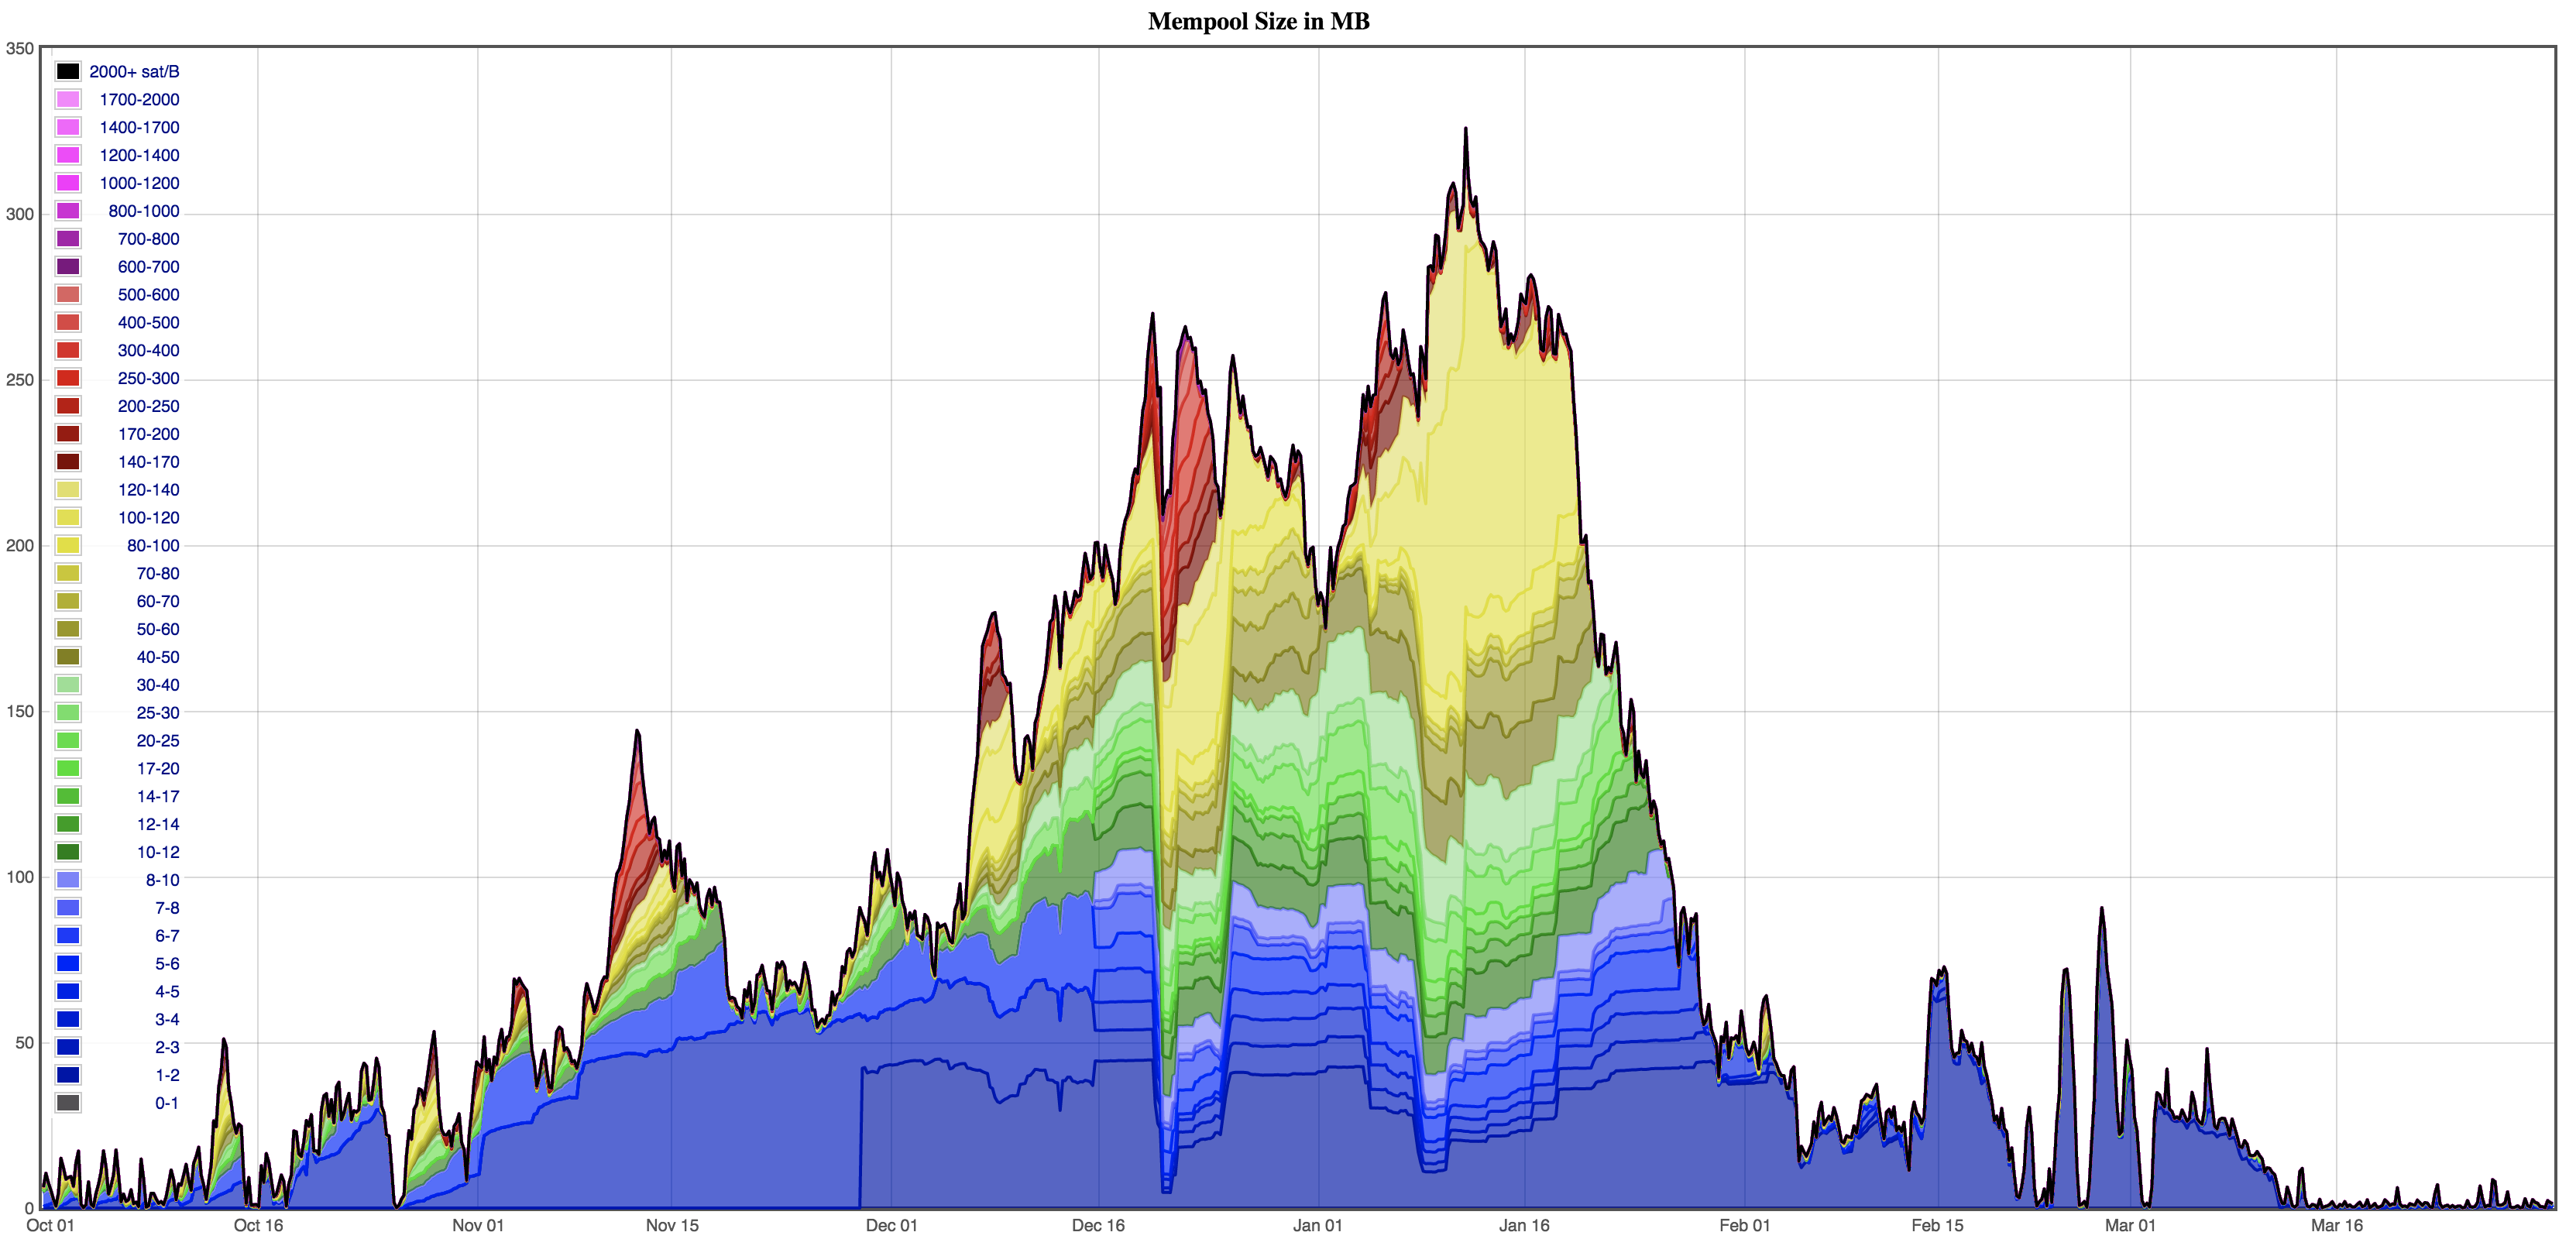
\includegraphics[height=5cm]{mempool.png}
    \end{center}
\end{frame}

\begin{frame}{Mempool}
    Le transazione in mempool NON vanno considerate come confermate.
\end{frame}

\section{Bibliografia}

\begin{frame}{Bibliografia} 
    \begin{itemize}
        \item Andreas M. Antonopoulos, "Mastering Bitcoin", 2015
        \item Adam Back, "Hashcash-a denial of service counter-measure", 2002
        \item Satoshi Nakamoto, "Bitcoin: A Peer-to-Peer Electronic Cash System", 2008
        \item Hal Finney, "Reusable Proofs of Work", 2004
    \end{itemize}
\end{frame}

\begin{frame}{Altre risorse} 
Tra le altre risorse utili mi piace citare:
    \begin{itemize}
        \item Ovviamente \href{https://t.me/BitPolimi}{BitPolimi} che ha organizzato queste lezioni.
        \item \href{http://satoshispritz.it}{Satoshi Spritz} - eventi serali a scadenze regolari per parlare di Bitcoin (a Milano ci incontriamo ogni mercoledì dalle 18).
        \item \href{https://t.me/ventunobtc}{Ventuno} - Podcast, raccolta di libri e materiali su Bitcoin.
        \item \href{http://officinebitcoin.it}{Officine Bitcoin} - lezioni su telegram da 30 minuti per la risoluzione di problemi pratici.
    \end{itemize}
\end{frame}


\begin{frame}{Domande} 
    \begin{center}
        
\includegraphics[height=5cm]{domande.jpg}
    \end{center}
\end{frame}

\begin{frame}[plain]
    \begin{center}
        
\includegraphics[height=8cm]{fine.jpg}
    \end{center}
\end{frame}

\end{document}
